\documentclass[paper=a5,pagesize=auto,twoside=false,fontsize=12pt,DIV=classic,BCOR=0mm,headinclude=true,footinclude=false]{scrbook}

%% font selection
\usepackage{utopia}
\usepackage{avant}

%% redefine headers
\usepackage[headsepline]{scrpage2}
\pagestyle{scrheadings}

\setkomafont{pageheadfoot}{%
  \normalfont\itshape
}

\automark[chapter]{chapter}
\renewcommand{\chaptermark}[1]{\markboth{#1}{#1}}
%\renewcommand{\sectionmark}[1]{\markright{#1}}

%% additional KOMA script options
\KOMAoptions{parskip=half,headsepline=true,numbers=noendperiod,captions=tableheading}
\recalctypearea{} % recalculate type area after selecting fonts

\usepackage{array}
\usepackage[british]{babel}
\usepackage{bbding}
\usepackage{float}  % direct positioning of floats
\usepackage{graphicx}
\usepackage{ifpdf}
\usepackage[utf8x]{inputenc}
\usepackage{paralist}
\usepackage{ucs}
\usepackage[obeyall]{siunitx}
\usepackage[hyphens]{url}
\usepackage{varioref}
\usepackage{wrapfig}  % must be included after package "float"

%% Make sure "hyperref" comes last of your loaded packages, to give it
%% a fighting chance of not being over-written, since its job is to
%% redefine many LATEX commands.
\ifpdf
	\usepackage[unicode,pdftex]{hyperref}
\else
	\usepackage[unicode,hypertex]{hyperref}
\fi

\hypersetup{
  unicode=true,                % non-Latin characters in Acrobat’s bookmarks
  pdftitle=K-Meter,            % title
  pdfauthor=Martin Zuther,     % author
  pdfsubject=K-Meter,          % subject of the document
  pdfcreator=Martin Zuther,    % creator of the document
  colorlinks=true,             % false: boxed links; true: colored links
  linkcolor=blue,              % color of internal links
  citecolor=blue,              % color of links to bibliography
  filecolor=blue,              % color of file links
  urlcolor=blue                % color of external links
}

%% KOMA script captions
\addtokomafont{caption}{\small}
\addtokomafont{captionlabel}{\bfseries}
\setcapindent{0em}

%% taken from package "l2tabu"
\tolerance 1414
\hbadness 1414
\emergencystretch 1.5em
\hfuzz 0.3pt
\widowpenalty=10000
\vfuzz
\hfuzz
\raggedbottom

%% package "varioref"
\labelformat{chapter}{chapter~#1}
\labelformat{section}{section~#1}
\labelformat{subsection}{section~#1}
\labelformat{subsubsection}{section~#1}

\labelformat{figure}{figure~#1}
\labelformat{table}{table~#1}

%% package "paralist"
\setdefaultitem{\textbullet}{$\circ$}{}{}

%% package "url"
\urlstyle{rm}

%% package "wrapfig"
\setlength{\intextsep}{0.2\baselineskip}

%% package "siunitx"
\sisetup{per=slash,trapambigfrac,locale=UK}

\newunit[unitspace=space]{\dB}{dB}
\newunit[unitspace=space]{\dBFS}{dB\,FS}
\newunit[unitspace=space]{\dBSPL}{dB\,SPL}
\newunit[unitspace=space]{\LK}{LK}
\newunit[unitspace=space]{\LKFS}{LK\,FS}

%% scaling of screenshots
\newcommand{\screenshotscale}{0.7}

%% layout
\usepackage[inner=18mm,outer=18mm,top=26mm,bottom=27mm,headsep=6.5mm,headheight=5mm]{geometry}

% %% start new page for every section
% \let\stdsection\section  
% \renewcommand\section{\newpage\stdsection}

%% command "application"
\DeclareRobustCommand*{\application}[1]{\texttt{#1}}


%%% Local Variables:
%%% mode: latex
%%% mode: outline-minor
%%% TeX-command-default: "Rubber"
%%% TeX-master: "../kmeter"
%%% TeX-PDF-mode: t
%%% ispell-local-dictionary: "british"
%%% End:

\hyphenation{
}


\title{K-Meter}
\author{Martin Zuther}
% edition 1.01

%% layout
\usepackage[inner=18mm,outer=18mm,top=26mm,bottom=27mm,headsep=6.5mm,headheight=5mm]{geometry}

\DeclareRobustCommand*{\application}[1]{\texttt{#1}}

\begin{document}

\title{K-Meter}

\subtitle{
  \normalsize{\textrm{\textmd{
        \vfill
        Free implementation of a K-System meter \\
        according to Bob Katz' specifications
        \vfill
        \begin{figure}[H]
          \centering{}
          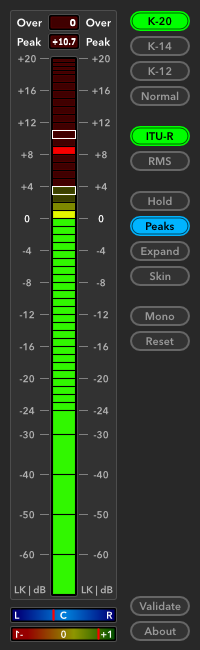
\includegraphics[scale=0.35,clip]{include/images/kmeter.png}
        \end{figure}
      }}}
}

\author{\normalsize\copyright{} 2010 Martin Zuther and contributors}
\date{}

\maketitle

\setcounter{tocdepth}{2}
\tableofcontents

\clearpage  % layout

\section{The loudness race}

When comparing two similar pieces of music, the louder one is
perceived as sounding better (although this is only true for short
periods of time).  Accordingly, the loudness of music productions has
continuously grown during the last decades.

As maximum levels of records, tapes and digital media are limited,
however, mastering engineers have started using sophisticated dynamic
compression techniques to achieve higher loudness without distorting
the music (as of 2010, distortion is increasingly being used in order
to achieve even higher loudness).

Unfortunately, this decrease in dynamic range does not leave the music
unharmed.  Current compressed music blasts away your ears and makes
you turn down the volume of your amplifier.  Having lowered the
volume, you'll find that the ``better-sounding'' compressed music
suddenly sounds pretty dull and boring compared to uncompressed music.
In contrast, music with high dynamic range makes you turn up the
volume -- heck, it even sounds better when broadcast on the radio!

\section{The K-System}

The K-System has been devised by mastering engineer Bob Katz in order
to counteract the ongoing loudness race and to help adjusting the
levels of different songs during mastering.  K-System meters are
average level meters that do \textbf{not} have 0\,dB on top.  Instead,
0\,dB on K-System meters relate to a reference loudness.  There are
three K-System scales:

\begin{compactitem}
\item K-20 (0\,dB at -20\,dBFS, recommended)
\item K-14 (0\,dB at -14\,dBFS)
\item K-12 (0\,dB at -12\,dBFS)
\end{compactitem}

Using the K-System is easy.  Just calibrate your monitor system so
that pink noise (-20\,dBFS RMS, 20\,Hz to 20\,kHz; see the K-Meter
source code for a FLAC-compressed wave file) on one channel yields
83\,dB\,SPL on a loudness meter set to \emph{C-weighted, slow}.  Then
mark the monitor's gain position as ``K-20''.

When your mixes or masters seem to have just the right loudness, they
should now yield 0\,dB on a K-20 meter.

In case you want to use the K-14 meter, attenuate the monitor gain by
6\,dB or repeat the above process so that pink noise yields
77\,dB\,SPL.  For K-12, attenuate the monitor gain by another 2\,dB
(pink noise should yield 75\,dB\,SPL).

For more information about the K-System, please see
\href{http://www.digido.com/level-practices-part-2-includes-the-k-system.html}{Bob's
  website}.

\section{Installation of K-Meter}

In order to use the pre-compiled binaries, please install the
``Fastest Fourier Transform in the West'' library first (see
\href{http://www.fftw.org/download.html\#platformspecific}{their
  website} for instructions).

When you're done, simply extract the K-Meter files from the downloaded
archive.  For the VST plug-in, you'll then have to move the extracted
files to your plug-in folder (\path{~/.vst}, \path{C:\Program
  Files\Steinberg\VstPlugins\} or the like).

\section{Controls}

\subsection{Meter selection}

\begin{figure}[H]
  \centering{}
  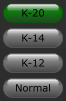
\includegraphics[scale=\screenshotscale,clip]{include/images/button_meter_selection.png}
\end{figure}


\subsection{Peak hold}

\begin{figure}[H]
  \centering{}
  
\includegraphics[scale=\screenshotscale,clip]{include/images/button_peak_hold_on.png} \\
  
\includegraphics[scale=\screenshotscale,clip]{include/images/button_peak_hold_off.png}
\end{figure}

\subsection{Peak meter}

\begin{figure}[H]
  \centering{}
  
\includegraphics[scale=\screenshotscale,clip]{include/images/button_peak_meter_on.png} \\
  
\includegraphics[scale=\screenshotscale,clip]{include/images/button_peak_meter_off.png}
\end{figure}

\subsection{Expand meter}

\begin{figure}[H]
  \centering{}
  
\includegraphics[scale=\screenshotscale,clip]{include/images/button_expand_meter_on.png} \\
  
\includegraphics[scale=\screenshotscale,clip]{include/images/button_expand_meter_off.png}
\end{figure}

\subsection{Mono switch}

\begin{figure}[H]
  \centering{}
  
\includegraphics[scale=\screenshotscale,clip]{include/images/button_mono_on.png} \\
  
\includegraphics[scale=\screenshotscale,clip]{include/images/button_mono_off.png}
\end{figure}

\subsection{Reset}

\begin{figure}[H]
  \centering{}
  
\includegraphics[scale=\screenshotscale,clip]{include/images/button_reset.png}
\end{figure}


\subsection{About}

\begin{figure}[H]
  \centering{}
  
\includegraphics[scale=\screenshotscale,clip]{include/images/button_about_on.png} \\
  
\includegraphics[scale=\screenshotscale,clip]{include/images/button_about_off.png}
\end{figure}

\subsection{License}

\begin{figure}[H]
  \centering{}
  
\includegraphics[scale=\screenshotscale,clip]{include/images/button_gpl_on.png} \\
  
\includegraphics[scale=\screenshotscale,clip]{include/images/button_gpl_off.png}
\end{figure}

\section{Meters}

\subsection{K-System meter}



\subsection{Overload counter}

\begin{figure}[H]
  \centering{}
  
\includegraphics[scale=\screenshotscale,clip]{include/images/overload_counter_normal.png} \\
  
\includegraphics[scale=\screenshotscale,clip]{include/images/overload_counter_clipped.png}
\end{figure}

\subsection{Maximum peak}

\begin{figure}[H]
  \centering{}
  
\includegraphics[scale=\screenshotscale,clip]{include/images/maximum_peak_normal.png} \\
  
\includegraphics[scale=\screenshotscale,clip]{include/images/maximum_peak_clipped.png}
\end{figure}

\subsection{Correlation meter}

\begin{figure}[H]
  \centering{}
  
\includegraphics[scale=\screenshotscale,clip]{include/images/correlation_meter.png}
\end{figure}

\subsection{Stereo meter}

\begin{figure}[H]
  \centering{}
  
\includegraphics[scale=\screenshotscale,clip]{include/images/stereo_meter.png}
\end{figure}

\section{Final words}

I love to hear from people who use my applications.  So if you can
spare the time, have any suggestions or want to create a nice theme,
head over to my website \href{http://www.mzuther.de/}{www.mzuther.de}
and drop me an email!

Finally, thanks for using free software.  I hope you'll enjoy this
experience \dots

\section{How to build K-Meter}

To build K-Meter yourself, you'll first have to install the
dependencies listed below.  To compile on 64-bit GNU/Linux operating
systems, you'll also have to install the multilib files for
\application{g++} (Debian package: \application{g++-multilib}).

\subsection{premake}

\begin{tabbing}
  \hspace*{6em}\=\=\kill

  Importance:  \> required \\
  Version:     \> 3.7 \\
  License:     \> GPL v2 \\
  Homepage:    \> \href{http://premake.sourceforge.net/}{premake.sourceforge.net}
\end{tabbing}

\subsection{premake4}

\begin{tabbing}
  \hspace*{6em}\=\=\kill

  Importance:  \> required \\
  Version:     \> 4.3 \\
  License:     \> GPL v2 \\
  Homepage:    \> \href{http://industriousone.com/premake}{industriousone.com/premake}
\end{tabbing}

\subsection{Fastest Fourier Transform in the West}

\begin{tabbing}
  \hspace*{6em}\=\=\kill

  Importance:  \> required \\
  Version:     \> 3.2.2 \\
  License:     \> GPL v2 \\
  Homepage:    \> \href{http://www.fftw.org/}{www.fftw.org}
\end{tabbing}

\subsubsection{Installation on GNU/Linux}

Extract the archive into the directory \path{libraries/fftw3}, change
into this directory and run:

\begin{verbatim}
  ./configure --enable-float CC="gcc -m32"
  make
  mkdir bin/
  mv .libs/* bin/
\end{verbatim}

\subsubsection{Installation on Microsoft Windows}

Extract the source code archive into the directory
\path{libraries/fftw3} and the archive containing the pre-compiled
binaries into the directories \path{libraries/fftw3/bin} and
\path (usually
  \path{C:\WINDOWS\system32\}).

\subsection{JUCE library}

\begin{tabbing}
  \hspace*{6em}\=\=\kill

  Importance:  \> required \\
  Version:     \> 1.51 \\
  License:     \> GPL v2 \\
  Homepage:    \> \href{http://www.rawmaterialsoftware.com/juce.php}{www.rawmaterialsoftware.com/juce.php}
\end{tabbing}

\subsubsection{Installation on GNU/Linux}

Extract the archive into the directory \path{libraries/juce}, change
into the directory \path{libraries/juce/build/linux/} and edit the
following lines in \path{juce_premake.lua} (please remove the
backslash characters and the corresponding line breaks):

\begin{verbatim}
  package.config["Debug"].target = "juce_debug32"
  package.config["Release"].target = "juce32"

  package.config["Debug"].buildoptions = \
    { "-D_DEBUG -ggdb -Wall -fPIC -m32" }
  package.config["Release"].buildoptions = \
    { "-fvisibility=hidden -fPIC -m32" }
\end{verbatim}

Finally, run:

\begin{verbatim}
  chmod +x runpremake
  ./runpremake
  make CONFIG=Debug
  make CONFIG=Release
\end{verbatim}

\subsubsection{Installation on Microsoft Windows}

Extract the archive into the directory \path{libraries/juce} and
compile the library.

\subsection{Virtual Studio Technology SDK (VST)}

\begin{tabbing}
  \hspace*{6em}\=\=\kill

  Importance:  \> optional \\
  Version:     \> 2.4 \\
  License:     \> proprietary \\
  Homepage:    \> \href{http://ygrabit.steinberg.de/}{ygrabit.steinberg.de}
\end{tabbing}

\subsubsection{Installation on GNU/Linux}

Extract the archive into the directory \path{libraries/vstsdk2.4}.

\subsubsection{Installation on Microsoft Windows}

Extract the archive into the directory \path{libraries/vstsdk2.4}.

\subsection{Building on GNU/Linux}

After preparing the dependencies, change into the directory \path{build} and
run

\begin{verbatim}
  ./run_premake
  make config=CFG TARGET
\end{verbatim}

where \application{CFG} is one of \application{debug32} and
\application{release32}, and \application{TARGET} is one of
\application{linux\_standalone} and \application{linux\_vst}.  The
compiled binaries will end up in the directory \path{bin}.

\subsection{Building on Microsoft Windows}

After preparing the dependencies, change into the directory
\path{build/windows/vs_2010}, open \path{kmeter.sln} with Visual C++
2010 and build the project.  The compiled binaries will end up in the
directory \path{bin}.

\end{document}


%%% Local Variables:
%%% mode: latex
%%% mode: outline-minor
%%% TeX-command-default: "Rubber"
%%% TeX-PDF-mode: t
%%% ispell-local-dictionary: "british"
%%% End:
